\subsection{Reactor Pattern}
\label{section:Reactor Pattern}

Das Reactor Pattern ist ein Design Pattern bei dem asynchrone auftretende Events, synchron abgearbeitet werden können. Dabei werden eingehende Nachrichten/Events von mehreren Clients sequentiell abgearbeitet. Durch das Reactor Pattern können nicht blockierende Applikationen entwickelt werden. Da das registrieren und aufrufen von Ereignissen vom Reactor Pattern übernommen wird gibt es eine lose Koppelung zwischen dem Lesen von I/O Operationen und der Applikation. \cite[p. 1]{Sch95}


\subsubsection{Motivation}
\label{section:reactor_motivation}

Douglas C. Schmidt beschreibt einen Anwendungsfall für das Reactor Pattern, bei dem Logging Informationen in einem Verteilten System an einen zentralen Server gesendet und gespeichert werden. Der Server soll in der Lage sein Logging informationen zu jederzeit speichern zu können und Logging Informationen können auch von mehreren Clients gleichzeitig an den Server gesendet werden. Möchte ein Client eine Verbindung zum Webserver aufbauen, wird der Thread des Webservers so lange blockiert, bis die Verbindung aufgebaut wurde und alle Daten übertragen wurden \cite[p. 1]{Sch95}. Sektion \ref{subsection: i/o speed} vergleicht wie lange I/O Operationen benötigen.

Eine Möglichkeit um mehrere Verbindungen auf einmal zu verarbeiten bietet Multithreading. Laut D. Schmit bringt diese Lösung jedoch folgende Probleme mit sich \cite[p. 2]{Sch95}:

\begin{itemize}
  \item Benötigt ein komplexes concurrency Schema
  \item Auf Single Core Prozessoren kann es zu einer schlechten Performance kommen
  \item Es könnte nicht auf allen Betriebssystemen verfügbar sein.
\end{itemize}

Die Nachteile 2 und 3 können 20 Jahre nach dem erscheinen dieses Papers als hinfällig angesehen werden, da mittlerweile multicore Prozessoren im Consumer Bereich angekommen sind und jedes relevante Betriebssystem Threads unterstützt. Das Problem Nummer 1 mit dem komplexen concurrency Schema bei der Verwendung von Multithreading bleibt bis heute bestehen.

\subsubsection{Funktionsweise}

Das Reactor Pattern implementiert eine Event Loop welche sich um das event demultiplexen und das event handler dispatchen kümmert. Dabei ist der Reactor ein Prozess mit einer endlosen Schleife (= Event Loop) der auf äußerde Ergebnisse reagiert. Um auf Ereignisse von außerhalb reagieren zu können müssen Callback Funktionen definiert werden, welche ausgeführt werden, wenn ein bestimmtes Ereignis eintritt. Dadurch kann eine Applikation auf die Ereignisse reagieren, für welche eine Callback Funktion definiert ist. In der Regel werden Callback Funktionen ausgeführt wenn eine blockierende I/O Operation abgeschlossen ist. Dabei können typische Ereignisse folgende sein \footnote{Die Liste ist angelehnt an folgenden Blog-Post: \url{http://pltconfusion.com/2014/10/20/eventmachine_internals_and_the_reactor_pattern/}}:

\begin{itemize}
  \item Eine Datei wurde von einem Filesystem gelesen
  \item Eine Datebank abfrage wurde gelesen
  \item Ein HTTP Request wurde kompletiert
\end{itemize}

Ob eine I/O Operation bereit abgeschlossen ist und dadurch nicht blockiert kann zum Beispiel über den Systemaufruf \emph{select} \footnote{Siehe auch Sektion \ref{section: Threads} Threads} bestimmt werden.

Der genaue Lebenszyklus des Reactor Patterns ist in Abbildung \ref{figure:reactor_cycle} beschrieben.

\begin{figure}[!htb]
  \centering
  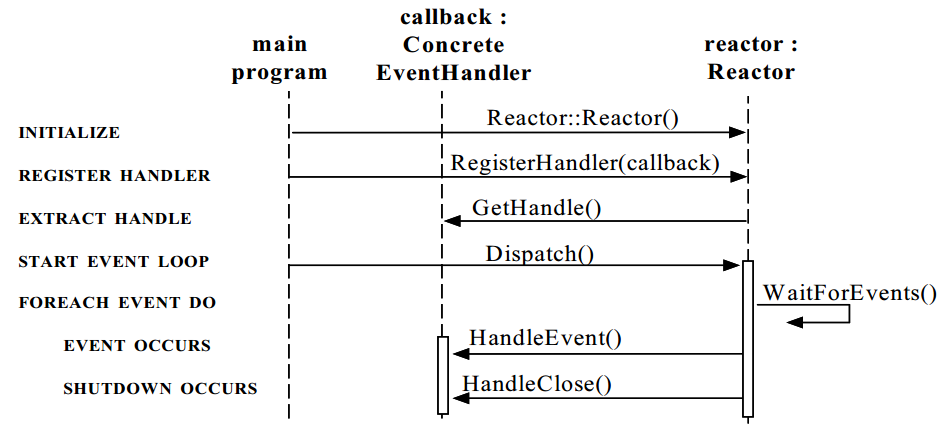
\includegraphics[width=13cm]{images/reactor.png}
  \caption{
    Zusammenarbeit der einzelnen Komponenten \cite[p. 5]{Sch95}
  }
  \label{figure:reactor_cycle}
\end{figure}

In der Initialisierung wird der Reactor in der main Methode erstellt. Nachdem ein Reactor erstellt wurde können sich unterschiedliche EventHandler beim Reactor registrieren. Diese EventHandler besitzten eine GetHandler Methode, welches die Callback Methode für ein Ereigniss zurückliefert. Sind alle Handler beim Reactor Registriert startet die Eventloop und wartet auf Ereignisse. Sobald ein Event eintritt wird die Callback Methode ausgeführt. Im letzten Schritt wird der Handler geschlossen und die Eventloop wartet auf die nächsten Ereignisse. 

Wie genau die Eventloop einzelne Ereignisse behandelt variiert zwischen den einzelnen Implementierungen. Eine Mögliche Implementierung ist das Ereignis an das Ende einer Queue zu geben und bei jedem durchlauf der Eventloop wird genau ein Ergebnis von der Queue genommen und behandelt.

Der Ablauf welcher in Abbildung \ref{figure:reactor_cycle} beschrieben ist richtet sich sehr an statischen Programmiersprachen wie C++.

Durch die Verwendung des Reactor Patterns wird eine enge Koppelung zwischen unabhängigen Teilen der Applikation und Applikations abhängigen teilen gelöst. Dadurch werden die Tief liegenden und komplexen Componenten wie das Demultiplexing von Events von der EventLoop übernommen. Durch die Verwendung von Events für blockierende Operationen wird der Programmierfluss vereinfacht da keine synchronisation der Daten nötigt ist \cite[p. 2]{Sch95}

\subsubsection{Reactor - Design Pattern}

Im folgenden werden die einzelnen Komponenten des Reactor Patterns genauer untersucht. In Abbildung \ref{figure:reactor_otm} wird die OTM Notation verwendet \footnote[0]{OTM ist der vorgänger von UML nährer Informationen findet man unter: \url{http://www.uml.org/}}.

\begin{figure}[!htb]
  \centering
  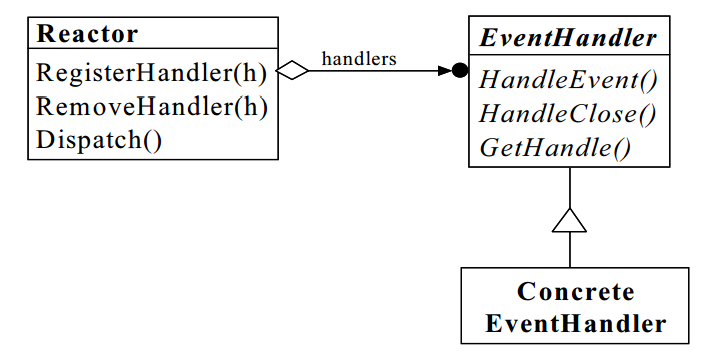
\includegraphics[width=9cm]{images/reactor_otm.png}
  \caption{
    Reactor OTM \cite[p. 4]{Sch95}
  }
  \label{figure:reactor_otm}
\end{figure}

\cite[p. 2]{Sch95}

\emph{Reactor:}
  Der Reactor für das registrieren, entfernen und dispatchen von Ereignissen verantwortlich. Die Eventloop welche Callback Methoden von Ereignissen ausführt befindet sich ebenfalls in dieser Klasse. Der Reactor ist Applikationsunabhängig und kann deswegen in anderen Applikationen wiederverwendet werden. 

\emph{Event Handler:}
	Die Eventhandler Klasse bietet ein Interface für einen konkreten EventHandler. In dynamischen Sprachen wie Ruby oder JavaScript welche keine Interfaces bieten kann diese Klasse hinfällig sein. 

\emph{ConcreteEventHandler}
	Der ConcreteEventHandler implementiert das Interface des Event Handlers. Dabei muss der Eventhandler folgende drei Methoden beinhalten: GetHandle, HandleEvent und StopEvent.

\subsubsection{Anwendungsgebiete}

Douglas Schmidt beschreibt in seiner Thesis folgende Anwendungsgebiete für das Reactor Pattern \cite[p. 4]{Sch95}:

\begin{itemize}
  \item Ein oder mehrere Ereignisse können gleichzeitig von unterschiedlichen Clients kommen
  \item Das Blockieren eines Clients oder das Pollen von Requests ist zu ineffizient
  \item Die gesendeten Nachrichten können in relativ kurzer Zeit verarbeitet werden
  \item Wenn unabhängige Teile der Applikation (Event Demultiplexing/Dispatching) von den abhängigen getrennt werden sollen
\end{itemize}

\subsubsection{Zusammenfassung}

Das Reactor Pattern bietet die Möglichkeit asynchron auftretende Ereignisse synchron abzuarbeiten. Um solche  bearbeiten zu können müssen sich Ereignisse beim Reactor mit einer Callback Funktion registrieren. Der Reactor verwendet eine endlose Schleife, welche eingetretene Ereignisse verarbeitet. Tritt ein Ereignis ein wird dieses einer Queue hinzugefügt. Bei einem der nächsten durchgängen der Eventloop wird die Callback Funktion des Ereignisses ausgeführt. 

Das Reactor Pattern findet seine Einsatz in Applikationen welche von blockierende I/O Operation abhängig sind. Bei solchen Applikationen tritt das Ereignis ein, wenn die I/O Operation beendet ist. Dadurch wird die CPU nicht blockiert und somit in keinen Ruhezustand versetzt. Durch den Systemaufruf \emph{select} kann überprüft werden ob eine Operation blockiert oder nicht. Dies kann vom Reactor Pattern verwendet werden um ein Ereignis auszuführen.